\documentclass{TUBthesis}

%%%%%%%%%%%%%%%%%%%%%%%%%%%%%%%%%%%%%%%%%%%%%%%%%%%%%%%%%%%%%%%%%%%%%%%%%%%%
% Predefined class variables
\Title{Grapheneinbettungen und Optimierung} %title of the thesis
\Thesis{Master Thesis} %type of thesis, i.e. bachelor/master/diploma
\Author{Jonas Neukamm} %name of author
%\Uni{Technische Universität Berlin}
\MNumber{324283} %matriculation number
\Supervisor{Prof. Dr. Stefan Felsner} %name of supervisor and first referee
\Referee{Dr. Frank Lutz} %name of second referee
\Date{7.6.2019} %date of delivery
\Language{german} %choose between english and german



%%%%%%%%%%%%%%%%%%%%%%%%%%%%%%%%%%%%%%%%%%%%%%%%%%%%%%%%%%%%%%%%%%%%%%%%%%%%
% Room for definiton of additonal commands or to include additional packages.
% Please check the loaded packages in the .cls file first.
\DeclareMathOperator*{\argmax}{arg\, max}
\usepackage{blindtext}
\usepackage[T1]{fontenc}
\usepackage{lmodern}
\usepackage{pgf,tikz}
\usepackage{amsmath,url}
\usepackage{enumitem}
\usetikzlibrary{patterns}
%\usepackage[demo]{graphicx}
\usepackage{caption}
\usepackage{subcaption}
%for algorithm
\usepackage{algorithm}
\usepackage{algpseudocode}
%bold symbols
\usepackage{bm}
\usepackage[textwidth=3.0cm]{todonotes}
\usepackage{capt-of}
%indicator function
\usepackage{dsfont}

%to ensure that floats stay in the subsection
\usepackage[section]{placeins}
\makeatletter
\AtBeginDocument{%
  \expandafter\renewcommand\expandafter\subsection\expandafter{%
    \expandafter\@fb@secFB\subsection
  }%
}
\makeatother

% footnotes
\usepackage[bottom]{footmisc}

% for nice looking tables
\usepackage{booktabs}
\newcommand{\ra}[1]{\renewcommand{\arraystretch}{#1}}


%for good refs
\usepackage{hyperref}
\usepackage{cleveref}
\usetikzlibrary{arrows}

%%%%proof: instead of proof.
\usepackage{xpatch}
\makeatletter

\xpatchcmd{\proof}{\@addpunct{.}}{\@addpunct{:}}{}{}

\AtBeginDocument{\xpatchcmd{\@thm}{\thm@headpunct{.}}{\thm@headpunct{}}{}{}}
\makeatother
% Math operators in correct font
\DeclareMathOperator{\vol}{Vol}
\DeclareMathOperator{\conv}{conv}
\DeclareMathOperator{\pos}{pos}
\DeclareMathOperator{\interior}{int}


%bigger than cdot, smaller than bullet \bigcdot
\makeatletter
\newcommand*\bigcdot{\mathpalette\bigcdot@{.5}}
\newcommand*\bigcdot@[2]{\mathbin{\vcenter{\hbox{\scalebox{#2}{$\m@th#1\bullet$}}}}}
\makeatother

 %For better figure placement
%
% Improved float placement parameters.
%
% From http://mintaka.sdsu.edu/GF/bibliog/latex/floats.html

% Alter some LaTeX defaults for better treatment of figures:
% See p.105 of "TeX Unbound" for suggested values.
% See pp. 199-200 of Lamport's "LaTeX" book for details.
% General parameters, for ALL pages:
\renewcommand{\topfraction}{0.95}	% max fraction of floats at top
\renewcommand{\bottomfraction}{0.95}	% max fraction of floats at bottom
% Parameters for TEXT pages (not float pages):
\setcounter{topnumber}{3}
\setcounter{bottomnumber}{2}
\setcounter{totalnumber}{4}     % 2 may work better
\setcounter{dbltopnumber}{2}    % for 2-column pages
\renewcommand{\dbltopfraction}{0.9}	% fit big float above 2-col. text
\renewcommand{\textfraction}{0.07}	% allow minimal text w. figs
% Parameters for FLOAT pages (not text pages):
\renewcommand{\floatpagefraction}{0.7}	% require fuller float pages
% N.B.: floatpagefraction MUST be less than topfraction !!
\renewcommand{\dblfloatpagefraction}{0.7}	% require fuller float pages


\begin{document}

\chapter{Einleitung}
Wir werden uns in dieser Arbeit mit Zeichnungen von einfachen planaren Graphen in der Ebene beschäftigen. Planare Graphen haben durch die Existenz kreuzungsfreier Einbettungen in gewissem Sinne besonders \glqq{schöne}\grqq{ } Zeichnungen. Aus diesem Grund ist eine der Fragen, mit der sich schon viele Mathematiker*innen auseinander gesetzt haben: \glqq\textit{How to draw a Graph?}\grqq\cite{tutte63}. Mit dieser Frage werden wir uns auch im nun Folgenden beschäftigen. 

Beginnen wir mit Varianten von Einbettungen, die wenige Einschränkungen haben. Bei einer topologischen Zeichnung eines planaren Graphen werden die Kanten als Kurven dargestellt. Hierbei dürfen sich die Kanten nur in den Knoten treffen. Erste mathematische Arbeiten hierzu zeigten, dass man diese Kurven auch als Geraden zeichnen kann. So wurde in den fünfziger Jahren des letzten Jahrhunderts unter anderem von István Fáry gezeigt, dass für jeden planaren Graphen und für jede Wahl eines äußeren Gebietes eine geradlinige und kreuzungsfreie Einbettung existiert \cite{fary48}.

In den siebziger Jahren des letzten Jahrhunderts betrachtete William Thomas Tutte die Unterklasse der 3-zusam\-men\-hängenden planaren Graphen und zeigte, dass für diese nicht nur geradlinige, sondern \textit{konvexe} Zeichnungen existieren \cite{tutte63}. Bei einer konvexen Einbettung bilden die Kantenfolgen, die ein Gebiet einschließen, die Randkurven von konvexen Polygonen.

\begin{figure}[h]
	\centering
  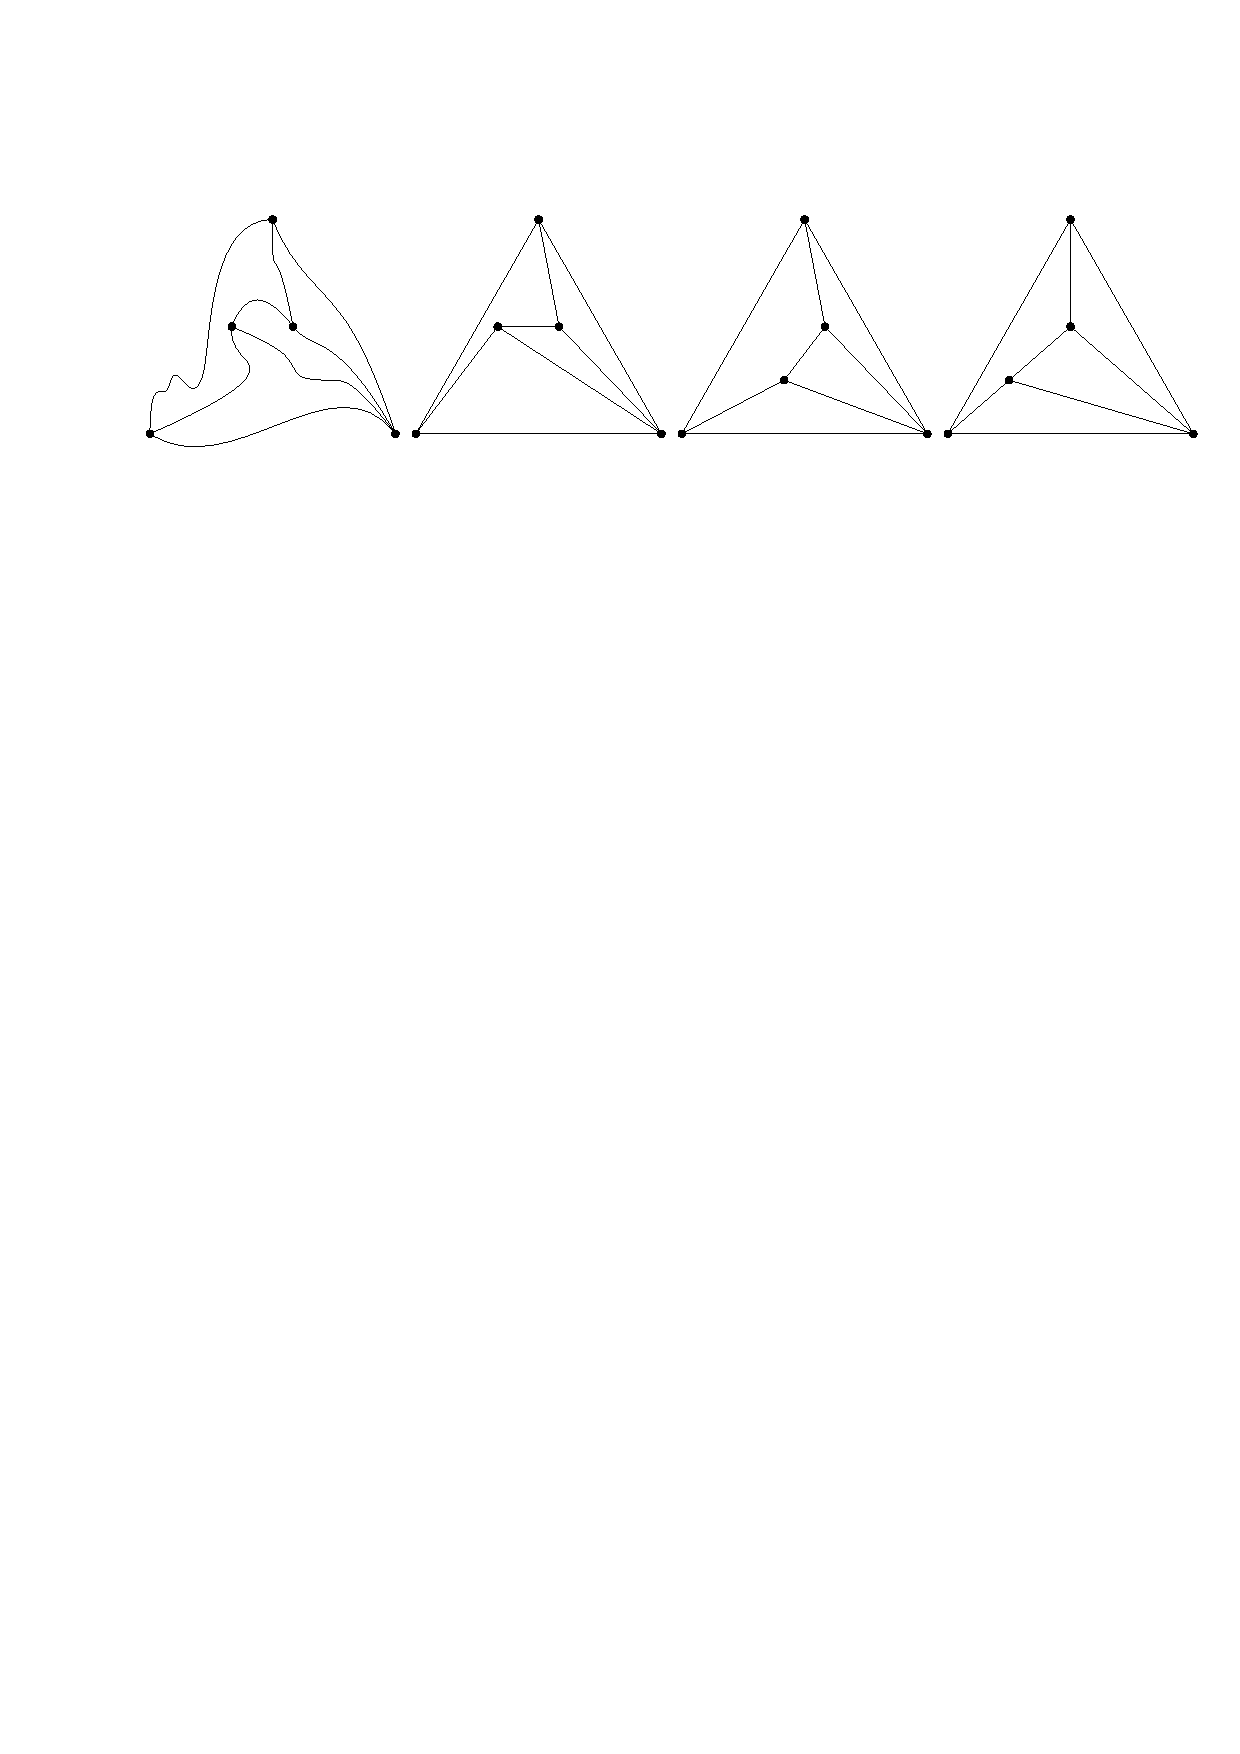
\includegraphics[width=1\textwidth]{topo_straight_convex.pdf}
	\caption{Der gleiche planare Graph mit einer topologischen, einer ge\-rad\-lini\-gen und einer konvexen Darstellung und unten rechts einer geradlinigen Dreiecks-Darstellung.}
	\label{topo_straight_convex}
\end{figure}

Im Weiteren folgt eine Auseinandersetzung mit einer spezifischen Form dieser Zeichnungen nach Nieke Aerts und Stefan Felsner. Wir fordern, dass alle Gebiete, inklusive dem Äußeren, nicht degenerierte Dreiecke einschließen. Wir nennen so eine Darstellung eine \textit{geradlinige Dreiecks-Darstellung}. Nicht alle planaren Graphen haben solche Zeichnungen, wie wir im Verlauf der Arbeit sehen werden. Man kann die Klasse der Graphen, die eine geradlinige Dreiecks-Darstellung zulassen, jedoch eingrenzen und Aerts und Felsner haben dies in einigen Publikationen getan \cite{af13h,af13,af15}.

Der Beitrag dieser Arbeit zum Thema liegt in der Implementierung eines von Aerts und Felsner entwickelten Algorithmus. Die Existenz einer geradlinigen Dreiecks-Darstellung wird in diesem als ganzzahlige Lösung eines Gerichteten-Multi-Fluss-Problems charakterisiert. Die Lösung eines solchen Problems ist im Allgemeinen NP-schwer. Experimentelle Rechenergebnisse legen aber den Schluss nahe, dass sich geradlinige Dreiecks-Darstellungen in polynomineller Zeit berechnen lassen. So kann man die Vermutung aufstellen, dass nicht-ganzzahlige Lösungen zu Berechnung von geradlinigen Dreiecks-Darstellungen genügen. Auch wenn wir den Beweis dieser Vermutung noch nicht gefunden haben, hilft sie bei der Beschleunigung des Algorithmus von Aerts und Felsner. Wir werden Indizien für die Korrektheit der Vermutung und mögliche Beweisansätze besprechen und zum Abschluss die Darstellung von errechneten geradlinigen Dreiecks-Darstellungen betrachten. 

Es folgt ein kurzer Überblick der Struktur der Arbeit. In Kapitel \ref{pre} wiederholen wir zunächst zum Verständnis der Arbeit wichtige Resultate aus der Graphentheorie und Optimierung. Kapitel \ref{main_theory} befasst sich mit notwendigen und hinreichenden Bedingungen für die Existenz von geradlinigen Dreiecks-Darstellungen. In Kapitel \ref{main_algo} wird aufbauend auf diesen Ergebnissen ein Algorithmus entwickelt, um eine geradlinige Dreiecks-Darstellung eines planaren Graphen zu berechnen, falls diese existiert. Abschließend wird in Kapitel \ref{the_program} ein Überblick über die Ergebnisse einer Implementierung des erarbeiteten Algorithmen gegeben.



\bibliographystyle{amsalpha}
\bibliography{bibliography}

\end{document}